\documentclass[11pt,a4paper]{article}

% --- Packages ---
\usepackage[utf8]{inputenc}
\usepackage[margin=1in]{geometry}
\usepackage[breaklinks=true,colorlinks,citecolor=blue,linkcolor=blue,urlcolor=blue]{hyperref}
\usepackage[table,xcdraw]{xcolor}
\usepackage{epsfig, mathrsfs, latexsym, subfigure, marginnote, gensymb, amsmath}
\usepackage{graphicx}
\usepackage{booktabs}
\usepackage{adjustbox}
\usepackage{doi}

% Package to handle multiple authors and affiliations cleanly in the article class
\usepackage{authblk}

% --- Metadata ---
\title{\textbf{pydemi: Interpretable Charge-Density Descriptors from DFT or Machine-Learned Densities, and What They Add to Materials Property Prediction}}

\author[1]{Shubham Kumar Maurya}
\author[1]{Somnath Bhowmick\thanks{bsomnath@iitk.ac.in}}
\affil[1]{Department of Materials Science \& Engineering, Indian Institute of Technology Kanpur, Kanpur 208016, India}

\date{\today}

% --- Document Start ---
\begin{document}

\maketitle

% --- ABSTRACT -------------------------------------------------------------
\begin{abstract}
The electronic charge density $\rho(\mathbf{r})$ of a density-functional theory
(DFT) calculation records the bonding that property models try to learn, but it
is rarely used directly as a model input. Learned representations of the
density grid predict properties well but have no individually interpretable
features, and the interpretable quantities of density analysis are computed one
structure at a time. We present pydemi, an open-source Python package that
reduces a VASP \texttt{CHGCAR}, and nothing else, to 56 fixed-length,
intensive and physically interpretable descriptors in three domains: bonding
(19), structural (19) and site heterogeneity (18). Every descriptor that would
need information a \texttt{CHGCAR} does not contain, or that is not converged on
typical VASP grids, has been left out, and each of the 56 is registered with its
formula, units, range and documented fallback values. When no DFT calculation
is available, pydemi predicts the density from the crystal structure with a
ChargE3Net model fine-tuned on our dataset, on the grid VASP would use; for 44
of the 55 informative descriptors the values computed from the predicted
densities of 605 held-out structures keep a rank correlation of at least 0.95
with their DFT values, and the critical-point counts are the main exception.
pydemi computes all descriptors of a 6,059-structure VASP dataset without a
failure in 8.4 CPU hours, is verified by 352 automated tests, and is used from
Python, the command line or a local graphical interface. Gradient-boosted
models trained on the descriptors alone predict 17 elastic, thermal,
energetic, electronic and optical properties of the same dataset, with test
$R^2$ of 0.85--0.95 for the moduli, elastic constants, thermal properties,
formation and cohesive energies and band gap, and a ROC-AUC of 0.984 for
metallicity. For the bulk, shear and Young's moduli ($R^2$ 0.949, 0.908 and
0.917) they are on par with graph neural networks trained on the same split
and ahead of every density-based neural network. Ten descriptors per property, chosen by their SHAP values on the training set, retain 92--99\% of the test $R^2$. The mean interstitial
density and the volume fraction of the non-covalent-interaction region are the
most important descriptors. Properties predicted from the descriptors of
ML-predicted densities agree with those from DFT densities (test $R^2$ for the
bulk modulus 0.958 against 0.956 on structures held out from both models), so
the whole path from a crystal structure to the properties runs without a DFT
calculation.
\end{abstract}

\section{Introduction}
\label{sec:intro}
The electronic charge density $\rho(\mathbf{r})$ is the central quantity of
density-functional theory: it determines the ground state and all of its
properties~\cite{hohenberg1964}, and it shows directly where electrons
accumulate between atoms, how much charge they transfer and how localized
they are. Every plane-wave DFT calculation produces it on a real-space grid,
and the Materials Project distributes such densities for a large and
continuously updated set of materials~\cite{jain2013,shen2022}. Most
machine-learning (ML) models of materials properties nevertheless do not use
them. Compositional featurizers compute statistics of elemental
properties~\cite{ward2016,ward2018}, and graph neural networks learn from the
atomic structure~\cite{xie2018,chen2019,choudhary2021,wen2024}; the bonding that
the density records is learned only implicitly.

Where the density has been used as a model input, it has mostly been as a
learned representation. Three-dimensional convolutional networks read the
density on a voxel grid~\cite{kajita2017,zhao2020} or its compressed latent
representation~\cite{kumar2026}, and persistent homology reduces it to Betti
curves over density thresholds~\cite{szymanski2025}. These representations
predict properties well, but their features have no individual physical
meaning, and the models must process the full grid of every structure. The
interpretable quantities of density analysis, on the other hand --- atoms and
critical points of the quantum theory of atoms in molecules~\cite{bader1990},
Bader charges~\cite{henkelman2006}, non-covalent interaction
regions~\cite{johnson2010} --- are computed by programs such as
critic2~\cite{oterodelaroza2014} and the Bader code~\cite{henkelman2006} that
are built to analyse one structure in depth. Their output is a list whose
length varies from structure to structure, not a fixed-length vector, and the
numerical choices behind it are left to the user.

Turning the density into fixed-length descriptors for many structures raises
three problems. The first is the input: the file that every VASP calculation
writes, the \texttt{CHGCAR}, does not support every quantity of density
analysis, and some it supports only with care: the
electron localization function and the local energy densities can be estimated
from a \texttt{CHGCAR} only through a density-only approximation of the kinetic
energy, several topological counts are not converged on typical grids, and the
PAW pseudo-density that a \texttt{CHGCAR} holds requires dedicated definitions.
A second obstacle is cost: a descriptor that needs a DFT density needs a DFT
calculation. Models that predict the density from the atomic
structure~\cite{chandrasekaran2019,jorgensen2022,koker2024} remove this
obstacle in principle, provided the descriptors survive the error of the
prediction. And the question that motivates the descriptors in the first place
--- how much of a material's properties they capture, and which of them carry
the information --- has to be answered on a common benchmark.

Here we describe pydemi, a Python package built around these three points. (i) It
reads one file, the VASP \texttt{CHGCAR}, and computes 56 descriptors that are
defined and numerically stable on it (Sections~\ref{sec:design}
and~\ref{sec:descriptors}); the analysis that led to the selection is
summarized in Section~\ref{sec:numerics}. (ii) It includes a density model, so
that the same descriptors are obtained from a crystal structure alone, and we
measure which descriptors transfer from DFT to predicted densities
(Section~\ref{sec:ml}). (iii) We train property models on the descriptors
alone for 17 properties of the 6,059 structures, compare them with structure-
and density-based neural networks on the same split, and identify the
descriptors that carry the information (Section~\ref{sec:properties}). The
package is used as a Python library, a command-line tool or a graphical
interface that runs locally (Section~\ref{sec:software}); the code, the tests
and the scripts that regenerate every number of this paper are released under
the MIT licence.

% ==========================================================================
\section{Design}
\label{sec:design}

\subsection{One input file}
pydemi reads the VASP \texttt{CHGCAR} (or \texttt{CHG}), plain or compressed:
the structure from its header and the total density from the first data block,
divided by the cell volume to give $\rho$ in e\,\AA$^{-3}$. Spin-polarized and
non-collinear files are accepted, and their magnetization blocks are ignored.
No \texttt{POTCAR}, \texttt{OUTCAR}, \texttt{AECCAR}, \texttt{ELFCAR} or
\texttt{LOCPOT} is needed. The restriction is deliberate: every VASP run writes
a \texttt{CHGCAR}, so any collection of calculations can be featurized without
returning to the original runs, and no descriptor depends on a file that is
present for some structures and missing for others. The shells and the power
partition use covalent radii tabulated in the package, and no descriptor needs
the valence electron count of the PAW datasets. Both input paths produce one
data model (Fig.~\ref{fig:architecture}): a \texttt{VolumetricData} object
that holds the structure, the density grid and a record of where the density
came from, which is written into the metadata of every output row.

\begin{figure}[htbp]
\centering
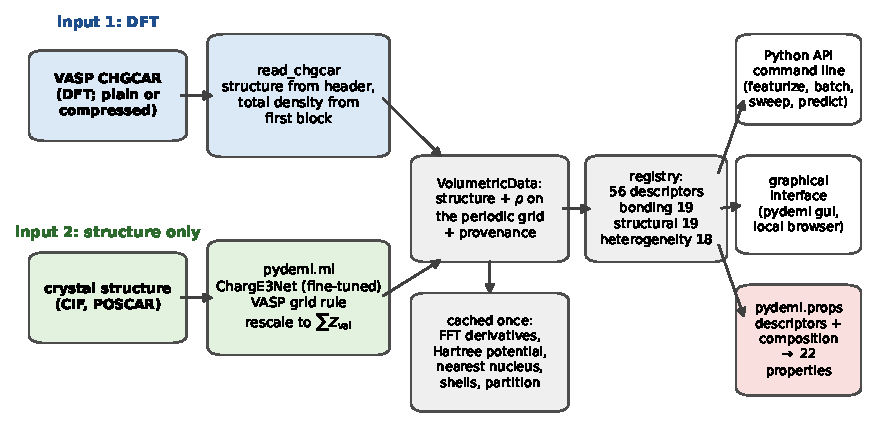
\includegraphics[width=\textwidth]{figures/fig_architecture.pdf}
\caption{Architecture of pydemi. A DFT \texttt{CHGCAR} and a crystal structure
whose density is predicted by the included ChargE3Net model give the same data
model; derived fields and the geometry pass are computed once per structure and
cached, and the registered descriptors reduce them. The descriptors are used
from Python, the command line or the graphical interface, and the property
models of Section~\ref{sec:properties} take them as input.}
\label{fig:architecture}
\end{figure}

\subsection{Numerical core}
Everything derived from the density is cached on the \texttt{VolumetricData}
object, keyed by the options it depends on, so that each field is evaluated
once per structure however many descriptors use it. Gradients, Hessians and
Laplacians are evaluated with the exact metric tensor of the cell,
$\nabla f=\sum_a\mathbf{b}_a\,\partial f/\partial u_a$ and
$\nabla^2 f=\sum_{ab}G_{ab}\,\partial^2 f/\partial u_a\partial u_b$ with
$G=BB^{\mathsf T}$ and $B$ the reciprocal basis, as exact derivatives of the
trigonometric interpolant (FFT, the default) or by central differences. The
Hartree potential follows from one Fourier transform of $\rho$. A single
geometry pass assigns every voxel its nearest nucleus, distance and direction,
with a periodic image search that is extended until it provably contains each
voxel's nearest image and a geometric tie-break for equidistant images. It
defines the core ($r\leq c_1$), bond ($c_1<r\leq c_2$) and interstitial
($r>c_2$) shells, with $c_1=0.8$ and $c_2=1.5$\,\AA{} by default or multiples of
the covalent radii. Three partitions --- nearest atom (the default), a power
diagram weighted by covalent radii, and Becke's fuzzy cells~\cite{becke1988}
--- share one interface that yields voxel--atom weights, so that every
site-resolved descriptor works with any of them.

\subsection{Descriptor registry}
Descriptors are plain functions registered with a decorator that records their
domain, the cached quantities they need, units, admissible range, references
and the values they return in degenerate cases. Registration enforces
intensivity: every count is per unit volume and every charge a fraction. A
degenerate input, such as a uniform density or a crystal in which no element
occupies two sites, returns a documented value together with a
\texttt{<name>\_\_flag} column instead of a bare NaN. The same registry
generates the descriptor catalogue, the reference document shipped with the
package and the parameter lists of the invariance tests, so that the three
cannot drift apart.

% ==========================================================================
\section{The 56 descriptors}
\label{sec:descriptors}

Table~\ref{tab:families} lists the descriptors by group; the formula and meaning
of each are given in Section~S1 of the Supporting Information and in the
reference document of the package. In what follows $k$ runs over the voxels,
$i(k)$ is the nearest nucleus of voxel $k$, $r_k$ its distance and
$\hat{\mathbf u}_k$ the unit vector from that nucleus to the voxel.

\begin{table}[htbp]
\centering
\caption{The 56 descriptors of pydemi by group.}
\label{tab:families}
\small
\begin{tabular}{p{3.2cm}rp{10.6cm}}
\toprule
Group & $n$ & Descriptors and what they measure \\
\midrule
\multicolumn{3}{l}{\emph{Bonding (19)}} \\
Moments and shells & 6 & $m_1$, $m_2$, $\sigma_r^2$: radial moments of the charge about its nearest nucleus; $f_\mathrm{core}$, $f_\mathrm{bond}$, $f_\mathrm{int}$: charge fractions in the three shells \\
Gradient anisotropy & 1 & $\zeta$: share of $\sum|\nabla\rho|$ that is not radial \\
Laplacian & 4 & volume and charge fractions where $\nabla^2\rho<0$; concentration ratio of the whole cell and of the valence region \\
Bond ellipticity & 1 & bounded ellipticity $1-\lambda_2/\lambda_1$ averaged over the bond shell \\
Non-covalent interactions & 3 & volume fraction of the NCI region~\cite{johnson2010}, its attractive share, mean of $\mathrm{sign}(\lambda_2)\rho$ \\
Hartree potential & 2 & spread of the site potentials; lowest interstitial potential \\
Bond midpoints & 2 & mean and spread of $\rho$ at the nearest-neighbour bond midpoints \\
\multicolumn{3}{l}{\emph{Structural (19)}} \\
Percolation & 4 & highest density level at which $\{\rho>c\}$ winds around the cell along each lattice vector; their anisotropy \\
Critical points & 4 & maxima and minima per volume; non-nuclear maxima and the charge in their basins \\
Density floor & 3 & $\rho_{\min}$, $\rho_{\min}/\langle\rho\rangle$, mean interstitial density \\
Anisotropy tensor & 4 & eigenvalues $t_1\le t_2\le t_3$ of $T_{ab}=\sum_k\partial_a\rho_k\partial_b\rho_k/\sum_k|\nabla\rho_k|^2$; fractional anisotropy \\
Information measures & 4 & Shannon entropy, disequilibrium, L\'opez-Ruiz--Mancini--Calbet complexity~\cite{lopezruiz1995}, Fisher information of $\rho/N_e$ \\
\multicolumn{3}{l}{\emph{Site heterogeneity (18)}} \\
Site statistics & 18 & for the per-site $m_1$, $f_\mathrm{bond}$ and $\zeta$: standard deviation, range, maximum, minimum, and the exact within/between-element split of the variance \\
\bottomrule
\end{tabular}
\end{table}

The bonding descriptors ask how the charge is arranged around the atoms and in
the bonds. The radial moments $m_n=\sum_k\rho_k r_k^n/\sum_k\rho_k$ and the shell
fractions describe how far the charge sits from its nearest nucleus; a large
interstitial fraction points to delocalized charge between the atoms. The
gradient anisotropy
\begin{equation}
\zeta = 1-\frac{\sum_k|\nabla\rho_k\cdot\hat{\mathbf u}_k|}{\sum_k|\nabla\rho_k|}
\end{equation}
vanishes for spherical, non-overlapping atoms and grows as charge is pulled off
the radial direction. The Laplacian descriptors locate where charge is
concentrated ($\nabla^2\rho<0$), the bounded ellipticity distinguishes
cylindrical from flattened charge in the bond shell, and the NCI descriptors
pick out the low-density, low-gradient regions of weak
interactions~\cite{johnson2010}. The structural descriptors treat the density of
the whole cell: how well it connects (percolation levels, detected by a
union--find over periodic images), its maxima, minima and non-nuclear maxima,
its floor, its directionality and its information content. The heterogeneity
descriptors turn per-site values of $m_1$, $f_\mathrm{bond}$ and $\zeta$ into
statistics over the atoms, including the decomposition
$\mathrm{Var}_iX=\sum_e x_e\mathrm{Var}_{i\in e}X+\sum_e x_e(\bar X_e-\bar X)^2$
into within- and between-element parts, where $x_e$ is the site fraction of
element $e$; the decomposition is exact, as in a one-way analysis of variance.

Every descriptor is invariant under supercell expansion, translation and rotation
of the crystal. One, the Laplacian concentration ratio
$\sum_{\nabla^2\rho<0}|\nabla^2\rho_k|/\sum_k|\nabla^2\rho_k|$, is identically
$\tfrac12$ for any periodic density, because the cell integral of
$\nabla^2\rho$ vanishes; over the dataset of Section~\ref{sec:dataset} it
differs from $\tfrac12$ by at most $2\times10^{-16}$. It is kept for continuity
with the original specification, and the same ratio restricted to the valence
region ($r_k>c_1$) carries the information. It is excluded from the analyses
below, which therefore use 55 informative descriptors.

% ==========================================================================
\section{What a CHGCAR supports}
\label{sec:numerics}

The 56 descriptors were selected from 220 candidates, which also covered
compositional, magnetic, electron-localization and energy-density quantities,
by evaluating every candidate on the dataset of Section~\ref{sec:dataset}. For
the 56 retained descriptors, the values in that evaluation agree with those of
the released package to a relative $10^{-8}$ for all 6,059 structures. Figure~\ref{fig:stability} collects the
sensitivity of each descriptor to the grid, the derivative scheme, the
partition and, for Section~\ref{sec:ml}, the prediction of the density by ML.

\begin{figure}[htbp]
\centering
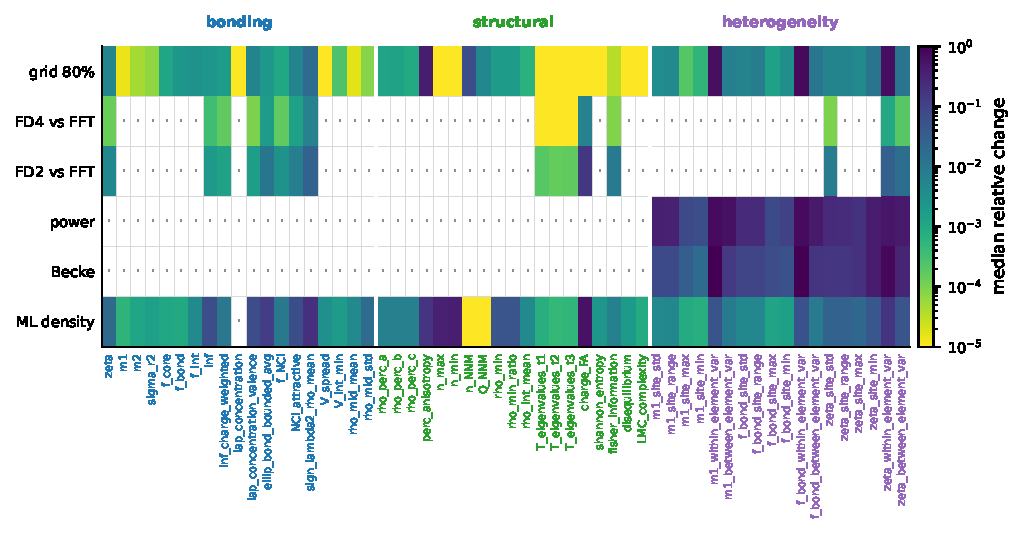
\includegraphics[width=\textwidth]{figures/fig_stability.pdf}
\caption{Sensitivity of the 56 descriptors (labels coloured by domain): median
relative change $|a-b|/\max(|a|,|b|)$ when the grid is Fourier-coarsened to
80\% of its points per axis (30 structures), when the FFT derivatives are
replaced by fourth- or second-order central differences (200 structures; 60 for
the site statistics of $\zeta$; 48 for the bounded ellipticity), when the
nearest-atom partition is replaced by the power diagram or Becke cells (300
structures), and when the descriptors are computed from the ChargE3Net
prediction instead of the DFT density (605 test structures,
Section~\ref{sec:ml}). Dots mark choices a descriptor does not depend on. The
Laplacian concentration ratio is constant (Section~\ref{sec:descriptors}). The
large values of the within-element variances on the coarsened grid and of the
percolation anisotropy reflect a near-zero reference value; those of the
heterogeneity descriptors under other partitions reflect a change of
definition.}
\label{fig:stability}
\end{figure}

\paragraph{Fields a CHGCAR does not provide.}
The electron localization function and the kinetic, potential and total energy
densities require the orbitals or, at least, the kinetic-energy density. A
\texttt{CHGCAR} contains neither, so these quantities would have to be
reconstructed from the PAW pseudo-density through a gradient expansion of the
kinetic energy~\cite{abramov1997,tsirelson2002}. The result is not the true
quantity, and its gradient anisotropy, which involves third derivatives of
$\rho$, changed by about 20\% between FFT and fourth-order derivatives and by
25\% on the coarsened grid. Magnetic
descriptors need the magnetization blocks, which the predicted densities of
Section~\ref{sec:ml} do not have, and compositional descriptors do not need the
density at all. These families are therefore left out of pydemi.

\paragraph{Descriptors not converged on VASP grids.}
The voxel-averaged ellipticity $\varepsilon=\lambda_1/\lambda_2-1$ diverges as
$\lambda_2\to0^-$ at bond-shell voxels away from the bond paths: its mean and
spread changed by a median 22\% and 67\% between fourth-order and FFT
derivatives. The bounded form $\varepsilon/(1+\varepsilon)=1-\lambda_2/\lambda_1$
changes by 0.21\% on the coarsened grid, 0.18\% with fourth-order and 1.2\% with
second-order derivatives, and is the only ellipticity in pydemi. The
saddle-point counts changed by a median 17--20\% on the coarsened grid, and a
grid census of critical points satisfied the Morse relation of the three-torus
for only 9.1\% of the structures; the counts of maxima and minima are kept, the
saddle counts are not.

\paragraph{Stability of the 56.}
Of the 55 informative descriptors, 46 change by at most 1\% (median) and 21 by
at most 0.1\% on the coarsened grid (Fig.~\ref{fig:stability}). Larger changes
occur for the percolation anisotropy (40\%), whose value is near zero for
every cubic cell, the non-nuclear maxima (6\%), and the within-element
variances (63--75\%), which are numerical noise of order
$10^{-9}$\,\AA$^2$ for the structures whose sites of each element are all
equivalent. For the 16 descriptors that use derivatives, fourth-order
differences agree with the FFT result to a median of $1.6\times10^{-4}$ and at
most $6\times10^{-3}$, so the FFT backend is the converged limit on these grids;
second-order differences shift them by up to 16\% (the fractional anisotropy of
$T$). The whole-cell descriptors do not depend on the partition. The 18 site
descriptors do, by definition: Becke cells, which like the nearest-atom
partition ignore atomic size, preserve the ranking of the structures by the
site standard deviations (Spearman $\rho_s=0.97$--0.99), whereas the power
diagram, which gives larger atoms larger cells, reorders them ($\rho_s$ down to
0.34). The partition is a setting of the interface and is recorded with every
result.

\paragraph{PAW pseudo-densities.}
A \texttt{CHGCAR} holds the pseudo-valence density plus the compensation charge
of the PAW method~\cite{blochl1994,kresse1999}, which is pseudized inside each
augmentation sphere. The density is negative somewhere in 61\% of the
structures, so $\rho_{\min}$ mostly reflects the pseudization, and pseudized
atoms can lack a maximum at the nucleus: 37\% of the structures have
non-nuclear maxima by the fixed 0.8\,\AA{} criterion, against 6\% when maxima
inside the augmentation spheres are excluded. pydemi keeps the fixed
criterion, because the augmentation radii are not part of a \texttt{CHGCAR},
and the reference document says so; the interstitial density and the
percolation levels, whose bottlenecks lie near the sphere radius where pseudo
and all-electron densities nearly agree, are not affected.

% ==========================================================================
\section{Validation}
\label{sec:validation}

pydemi is tested by 352 automated tests (Table~\ref{tab:validation}; each is
described in Section~S6 of the Supporting Information). Nearly half of
them, 169, form an invariance harness that is parametrized over the registry:
every descriptor is computed for a low-symmetry model crystal and for its
$2\times2\times2$ supercell, a translation of the origin and a rigid rotation,
and must agree to $10^{-6}$ relative, so that descriptors added later are
checked automatically. The other library tests compare with closed forms for
Slater and Gaussian densities, exact identities and brute-force references; the
model tests check that the included ChargE3Net code reproduces the original
implementation, and the interface tests run the graphical interface end to end
for both inputs and the comparison of the two densities. The continuous-integration
workflow runs the suite on Linux, macOS and Windows with Python 3.10--3.13, with
and without the optional extras, together with a strict static type check and a
test of the built package.

\begin{table}[htbp]
\centering
\caption{Checks of the test suite and the accuracy required.}
\label{tab:validation}
\small
\begin{tabular}{p{4.0cm}p{8.0cm}r}
\toprule
Check (tests) & Content & Tolerance \\
\midrule
Invariance harness (169) & every descriptor under a $2\times2\times2$ supercell, a translation and a rotation & $10^{-6}$ rel. \\
Derivatives (16) & FFT exact for band-limited functions in a triclinic cell; finite-difference convergence order; Hessian trace = Laplacian & $10^{-9}$--$10^{-10}$ \\
Geometry and partitions (18) & nearest-image distances against brute force, including an extreme shear; partitions of unity; charge conservation & $10^{-12}$ \\
Closed forms and identities (40) & radial moments of Slater densities; percolation of a simple cubic lattice at the midpoint density; known critical points; variance decomposition; Laplacian concentration $=\tfrac12$; Hartree potential of a Gaussian & $10^{-2}$--$10^{-12}$ \\
Input, batch and tooling (21) & \texttt{CHGCAR} layouts (1, 2, 4 blocks, VASP 4/5), volume scaling; fixed batch schema; no bare NaN; float32 against float64 & exact / reported \\
Density model (13) & VASP grid rule; neighbour lists against brute force; predictions equal the original ChargE3Net code, independent of chunking, invariant to rotation and permutation; renormalization & $10^{-5}$ of $\rho_{\max}$ \\
Property models (12) & stored test predictions reproduced, also by the 22 distributed models; range checks & $10^{-9}$ rel. \\
Graphical interface (63) & end-to-end runs for both inputs and the comparison view; every descriptor has a figure whose plotted data reproduce its value & $10^{-7}$ rel. \\
\bottomrule
\end{tabular}
\end{table}

% ==========================================================================
\section{Application to a 6,059-structure DFT dataset}
\label{sec:dataset}

The dataset, introduced in Ref.~\cite{kumar2026}, comprises 6,059 VASP charge
densities of 87 elements, computed for relaxed structures from the Materials
Project: 86 elemental solids, 3,195 intermetallics and 2,778 compounds with
electronegative elements. The 4,901 runs that include their \texttt{OUTCAR}
share one protocol: single-point VASP~\cite{kresse1996} calculations with the
PBE functional~\cite{perdew1996} and one PAW dataset~\cite{kresse1999} per
element, a 500\,eV plane-wave cutoff, collinear spin polarization and an
automatic $k$-mesh. The cells contain 1--152 atoms (median 6) on grids of
$1.8\times10^5$ to $1.7\times10^6$ points (5th--95th percentile).

pydemi computed the 56 descriptors of every structure without a failure, in
37 minutes on 16 worker processes (8.4 CPU hours in total). The median cost is 3.3\,s per
structure (95th percentile 15\,s); it follows the number of grid points
(Spearman 0.96) more closely than the number of atoms (0.77). On one core a
6\,MB \texttt{CHGCAR} on a $56^3$ grid takes 0.7\,s and 0.25\,GB, and a
350\,MB one on a $216^3$ grid 54\,s and 2.6\,GB, including the data for the
figures of the graphical interface. For 421 structures no element
occupies two sites, and their within-element variances return the documented
NaN with a flag.

% ==========================================================================
\section{Descriptors from the crystal structure alone}
\label{sec:ml}

\subsection{The density model}
pydemi includes ChargE3Net~\cite{koker2024}, an E(3)-equivariant network that
predicts the density at arbitrary points from the atomic structure, adapted to
predict one structure at a time on any device, with the published architecture
unchanged (three interaction layers, $l_{\max}=4$, 4\,\AA{} cutoff;
1.9 million parameters). The checkpoint shipped with the package (8\,MB) was
fine-tuned for 50,000 steps from the published Materials Project checkpoint on
the VASP densities of the dataset, with 5,152 structures for training, 302 for
validation and 605 for testing. The published checkpoint itself is not usable on
this dataset, because several of its PAW datasets, and hence its valence counts,
differ from ours. A prediction stands for a \texttt{CHGCAR} computed with the
settings of the dataset. Its grid is the one VASP would use: along each
lattice vector $\mathbf a_i$ the wavefunction grid is the smallest even size
with prime factors 2, 3, 5 and 7 that is at least $\mathrm{nint}(2w\,x_i)$,
with $x_i=|\mathbf a_i|\sqrt{E_{\mathrm{cut}}/\mathrm{Ry}}/2\pi$ in atomic units
and $w=2$ for accurate precision, and the density grid is twice that; for
$E_{\mathrm{cut}}=500$\,eV the rule reproduces the grids of all 6,059
calculations. The predicted density is rescaled to the valence electron count
of the PAW datasets of the training data (87 elements), and the model, the
checkpoint hash and the scale factor are recorded with the result. The
included code reproduces the predictions of the original implementation to
$6\times10^{-7}$ of the peak density for the structures we checked, and its cost
grows with the number of atom--grid-point pairs within the cutoff, about
0.35\,ms per pair on one CPU core; a GPU is used when one is available.

\subsection{Transfer of the descriptors}
On the full DFT grids of the 605 test structures the predictions have a
normalized mean absolute percentage error (NMAPE) of 0.72\% on average (median
0.58\%); structures with lanthanides or actinides are predicted less
accurately, and the worst case, YbPrZn$_2$, has 10.4\%. Before rescaling, the
predicted densities integrate to the nominal electron count within 0.13\%
(median; largest deviation 1.5\%). All 605 were featurized without error.

\begin{figure}[htbp]
\centering
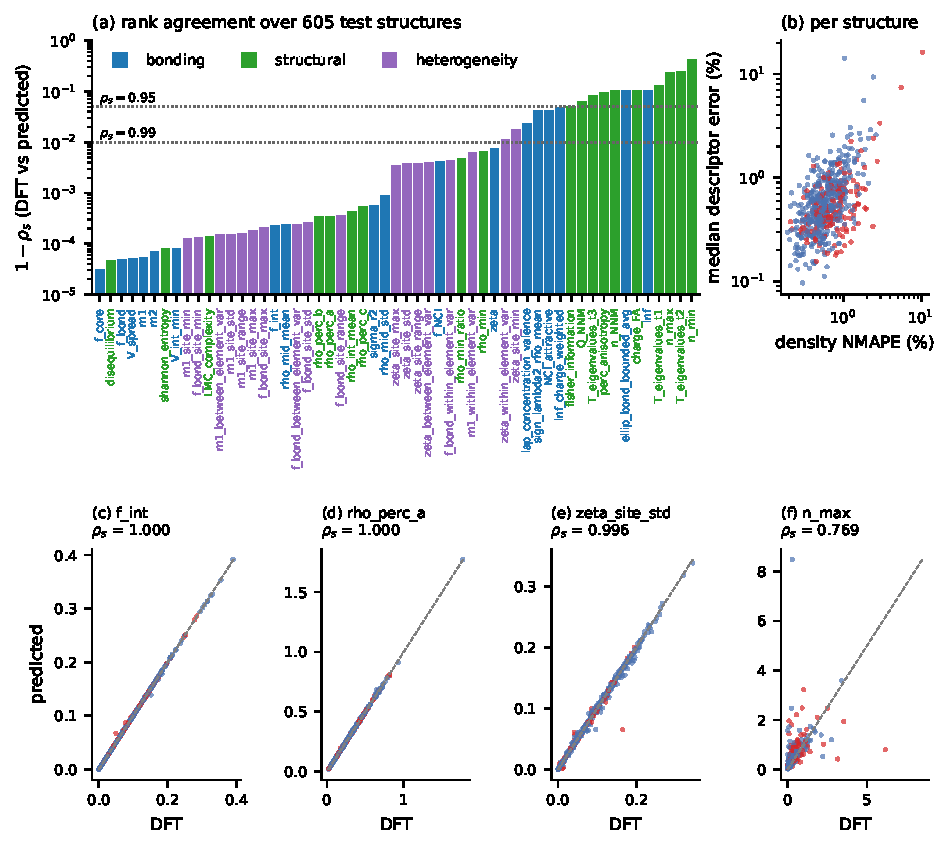
\includegraphics[width=\textwidth]{figures/fig_ml.pdf}
\caption{Descriptors of predicted densities (605 test structures of the density
model). (a) Rank disagreement $1-\rho_s$ between the descriptors of the DFT and
the predicted densities for the 55 informative descriptors; dotted lines mark
$\rho_s=0.99$ and 0.95. (b) Median relative error per structure over the 44
descriptors with $\rho_s\geq0.95$ against the density error. (c--f) Predicted
against DFT values for three descriptors that transfer and one that does not;
red: structures containing lanthanides or actinides.}
\label{fig:ml}
\end{figure}

For 44 of the 55 informative descriptors the rank correlation between the
values from the DFT and the predicted densities across the test structures is
at least 0.95, and for 37 it is at least 0.99 (Fig.~\ref{fig:ml}a); over all 55
the median relative error is 0.66\%. The descriptors that transfer include all
18 heterogeneity descriptors, 16 of the 18 informative bonding descriptors (the
moments and shell fractions, $\zeta$, the NCI and potential descriptors and the
bond-midpoint densities), and the percolation levels, density floor and
information measures (Fig.~\ref{fig:ml}c--e). The 11 that do not fall into
three groups. The counts of maxima and minima ($\rho_s=0.77$ and 0.57, median
errors 35\% and 38\%) respond to shallow spurious extrema in flat, low-density
regions (Fig.~\ref{fig:ml}f); the non-nuclear maxima and their charge
($\rho_s=0.90$ and 0.94) are zero in both densities for 61\% of the structures,
so their ranks are dominated by ties. The bounded ellipticity and the
negative-Laplacian volume fraction (median errors 13\% and 6\%) involve second
derivatives in low-density regions, which amplify the short-wavelength error of
the prediction. The eigenvalues of the anisotropy tensor, its fractional
anisotropy and the percolation anisotropy are predicted accurately
($R^2\geq0.987$; median error of the eigenvalues at most 0.07\%), but their
values cluster, for instance at $\tfrac13$ for every cubic cell, so that small
errors reorder them. Per structure, the median error over the 44 transferable
descriptors is 0.53\% (90th percentile 1.2\%) and follows the density error
(Spearman 0.49; Fig.~\ref{fig:ml}b); it exceeds 5\% only for Ba$_3$N, Li,
TiH$_2$, Yb$_2$MgIn and YbPrZn$_2$. One limitation remains: the model predicts the
total density only, so pydemi offers no magnetic descriptors on this path, as
on the DFT path.

% ==========================================================================
\section{Property prediction}
\label{sec:properties}

\subsection{Data and protocol}
The targets of the 6,059 structures come from two sources. The bulk, shear and
Young's moduli, and an energy per atom relative to the free atoms together with
a Debye temperature, are those used in the cross-model benchmark of
Ref.~\cite{maurya2026}. The other properties were retrieved from the Materials
Project (database version 2026.04.13) for the same material
identifiers~\cite{jain2013}: the elastic constants $C_{11}$, $C_{12}$ and
$C_{44}$~\cite{dejong2015}, kept only where the stiffness tensor is Born-stable
and the moduli agree with those of the benchmark; the Debye temperature, sound
velocities and minimum thermal conductivities in the Clarke and Cahill
models~\cite{clarke2003,cahill1992} derived from the elastic data; the formation
and cohesive energies; the PBE band gap, metallicity and directness of the gap;
and the refractive index~\cite{petousis2017}, available for 1,362 materials. The
train/validation/test split is the one of the benchmark (4,847/606/606
structures); a material without a value is left out for that property only.

The inputs of every model are the 55 informative pydemi descriptors (the
Laplacian concentration ratio, which is $\tfrac12$ for every structure, is left
out). For each property we trained ridge regression (logistic regression for the
two classifications), random forests with 500 trees~\cite{pedregosa2011} and
LightGBM~\cite{ke2017}. The LightGBM hyperparameters (learning rate, number of
leaves, minimum leaf size, feature and bagging fractions, $L_1$ and $L_2$
penalties) were tuned with 50 trials of the tree-structured Parzen estimator of
Optuna~\cite{akiba2019} on the validation loss, with early stopping on the
validation set and at most 10,000 boosting rounds. The refractive index, which
is heavy-tailed, was modelled on a logarithmic scale. The random forests and
the tuned LightGBM models were refit with five seeds; we report the mean and
standard deviation of the test metrics over the seeds. The test set was used
only for the final evaluation. Feature importance is the mean absolute SHAP
value~\cite{lundberg2020} on the test set. To measure how concentrated the
information is, every model was also retrained, with the same protocol, on only
the ten descriptors with the largest mean absolute SHAP value of its LightGBM
models on the training set, so that the test set plays no part in their choice.

\subsection{Accuracy}
Table~\ref{tab:properties} and Fig.~\ref{fig:properties}a give the test scores
of LightGBM, which was the most accurate of the three models for every property
(for the direct-gap classification the random forest was better by 0.001;
Supporting Information, Table~S3). With the descriptors alone, the models reach
$R^2$ of 0.949, 0.908 and 0.917 for the bulk, shear and Young's moduli,
0.87--0.92 for the elastic constants, 0.85--0.93 for the Debye temperature,
the sound velocities and the minimum thermal conductivities, 0.922 and 0.887
for the formation and cohesive energies and 0.852 for the band gap.
Metallicity is classified with a ROC-AUC of 0.984 (accuracy 0.940) and the
directness of the gap, known for only 1,645 materials, with 0.787 (accuracy
0.795). The refractive index, for which only 1,089 training materials are
available, reaches $R^2=0.758$. The seed-to-seed standard deviation is at most
0.005, except for the band gap (0.015) and the refractive index (0.011).

\begin{table}[htbp]
\centering
\caption{Test scores of tuned LightGBM models on the pydemi descriptors: $R^2$,
or ROC-AUC for the two classifications, mean $\pm$ standard deviation over five
seeds, with all 55 informative descriptors and with the ten most important
descriptors of each property. MAE: mean absolute error with the 55
descriptors. $n$: training and test materials.}
\label{tab:properties}
\begin{adjustbox}{width=\textwidth}
\begin{tabular}{llrrccr}
\toprule
Property & Units & $n_\mathrm{train}$ & $n_\mathrm{test}$ & 55 descriptors & 10 descriptors & MAE \\
\midrule
\csname @@input\endcsname tables/tab_properties.tex
\bottomrule
\end{tabular}
\end{adjustbox}
\end{table}

\begin{figure}[htbp]
\centering
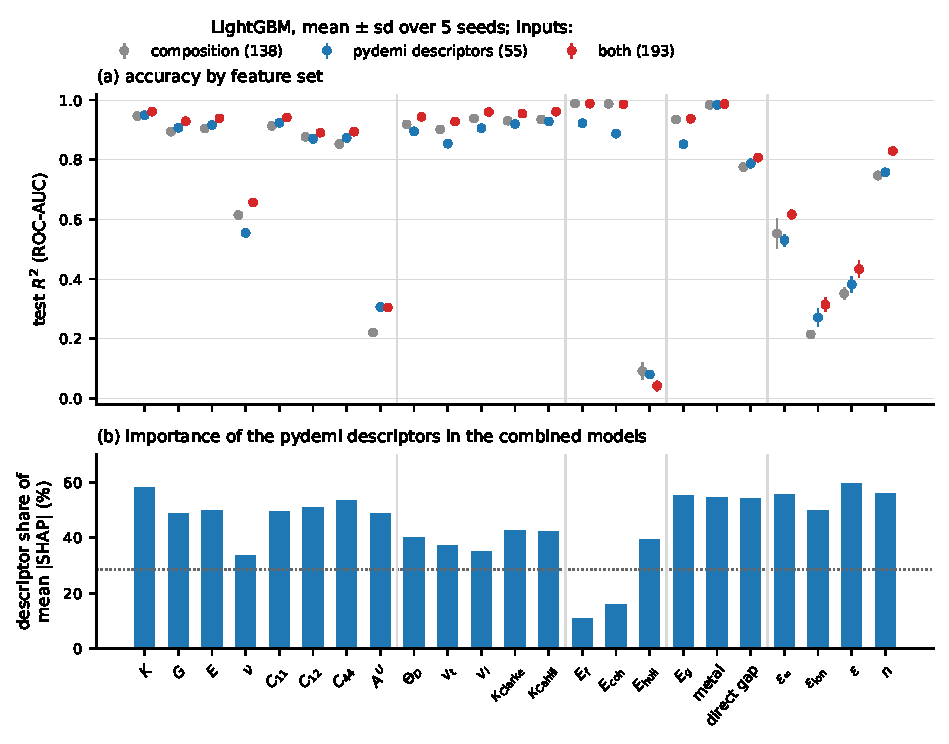
\includegraphics[width=\textwidth]{figures/fig_properties.pdf}
\caption{(a) Test scores of LightGBM on the 55 pydemi descriptors and on the
ten most important descriptors of each property (mean and standard deviation
over five seeds; ROC-AUC for metallicity and the direct gap). (b) Share of the
mean absolute SHAP value of the 55-descriptor models carried by the eight
descriptors that are most important over all properties.}
\label{fig:properties}
\end{figure}

\subsection{Comparison with neural networks on the same split}
Ref.~\cite{maurya2026} trained graph neural networks on the crystal structure
(CGCNN~\cite{xie2018}, MEGNet~\cite{chen2019}, the equivariant
MatTen~\cite{wen2024}), a convolutional network on the latent representation of
the full density grid (LatentMatFusion~\cite{kumar2026}), MatTen with the density
fused into the structure, and ChargE3Net~\cite{koker2024} adapted to property
regression, all on the split used here, for five targets
(Table~\ref{tab:benchmark}). For the three moduli, LightGBM on the descriptors,
55 numbers per structure, is on par with the graph networks ($R^2$ 0.949, 0.908
and 0.917 against 0.961, 0.908 and 0.920 for CGCNN and 0.953, 0.880 and 0.888
for MEGNet) and ahead of every model in Ref.~\cite{maurya2026} that uses the
density (at most 0.940, 0.888 and 0.902). For the Debye temperature of the
benchmark ($R^2=0.908$) it is behind CGCNN, MEGNet and ChargE3Net
(0.918--0.938) and ahead of the other three models. For the energy relative to
the free atoms ($R^2=0.860$) it is behind every model (0.880--0.987): this
energy depends on the free-atom reference of each element, which the
descriptors, intensive features of the density, do not identify, whereas every
neural network of the benchmark knows the elements. With only ten descriptors per property, LightGBM still reaches $R^2$ of 0.937, 0.875 and 0.890 for the three moduli, above two of the three density-based networks for each. The models in
Ref.~\cite{maurya2026} were trained once each, and for the energy and the Debye
temperature the test sets here contain the 592 and 476 test materials with a
value; the comparison is therefore indicative at the level of 0.01 in $R^2$.

\begin{table}[htbp]
\centering
\caption{Test $R^2$ and MAE for the five properties of the cross-model benchmark
of Ref.~\cite{maurya2026} on the same split. MAE in GPa for $K$, $G$, $E$, eV/atom
for $E_\mathrm{form}$ (energy relative to the free atoms) and K for $\Theta_D$.
Upper block: this work, LightGBM on the pydemi descriptors, mean over five
seeds (test materials: 606, 606, 606, 592 and 476). Lower block: as reported in
Ref.~\cite{maurya2026}. $^\dagger$Equal to the MAE of $G$ in the source; as
reported.}
\label{tab:benchmark}
\begin{adjustbox}{width=\textwidth}
\begin{tabular}{lcccccccccc}
\toprule
Model & \multicolumn{2}{c}{$K$} & \multicolumn{2}{c}{$G$} & \multicolumn{2}{c}{$E$} & \multicolumn{2}{c}{$E_\mathrm{form}$} & \multicolumn{2}{c}{$\Theta_D$} \\
\cmidrule(lr){2-3} \cmidrule(lr){4-5} \cmidrule(lr){6-7} \cmidrule(lr){8-9} \cmidrule(lr){10-11}
 & $R^2$ & MAE & $R^2$ & MAE & $R^2$ & MAE & $R^2$ & MAE & $R^2$ & MAE \\
\midrule
\csname @@input\endcsname tables/tab_benchmark.tex
\bottomrule
\end{tabular}
\end{adjustbox}
\end{table}

\subsection{Which descriptors carry the information}
The most important descriptor overall is the mean interstitial density. It is
the most important input for the bulk modulus (28\% of the mean absolute SHAP
value), the shear and Young's moduli, the three elastic constants and the
refractive index (Fig.~\ref{fig:properties}b). The volume fraction of the NCI
region has the same role for the electronic properties: it is the most
important input for the band gap (31\%), metallicity (30\%) and the formation
energy (19\%). For the Debye temperature, the sound velocities and the minimum
thermal conductivities, the radial spread $\sigma_r^2$, the interstitial charge
fraction and the valence Laplacian concentration lead, and the cohesive energy
draws on the bond-midpoint and interstitial densities. Only the direct-gap
classification has no dominant descriptor (at most 7\%). The information is concentrated in few descriptors: the ten most important
descriptors of a property (ranked on the training set; Supporting Information,
Table~S4) carry 46--69\% of its mean absolute SHAP value, and models trained on
these ten alone lose 0.01--0.07 in $R^2$ (Table~\ref{tab:properties},
Fig.~\ref{fig:properties}a), least for the bulk modulus (0.937 against 0.949),
$C_{12}$ and metallicity, most for the transverse sound velocity (0.782 against
0.854), the band gap and the cohesive energy. Only 34 of the 55 descriptors
appear in any of the 17 lists; the mean interstitial density (in 16 lists), the
radial spread $\sigma_r^2$ (14) and the negative-Laplacian volume fraction (13)
appear most often. Six to nine (on average 8.4) of the ten descriptors of each
property transfer to predicted densities with $\rho_s\geq0.95$
(Section~\ref{sec:ml}), so the information the models use is largely the
information that survives the density model.

\subsection{From a crystal structure to properties}
For the 605 test structures of the density model we evaluated the property
models (LightGBM, seed 0) with the descriptors of the predicted densities in
place of the DFT ones. The two predictions agree: $R^2$ between them is 0.985
for the bulk modulus, 0.950 and 0.955 for the shear and Young's moduli,
0.950--0.975 for the elastic constants, 0.930--0.971 for the thermal
properties, 0.964 and 0.935 for the formation and cohesive energies, 0.956 for
the band gap and 0.959 for the refractive index; the metallicity class is the
same for 98.2\% of the structures. Sixty-three of these structures are also in
the test set of the property models, so that neither model saw them in
training. On these 63, the bulk modulus predicted from the ML descriptors has
$R^2=0.958$ (MAE 10.9\,GPa), as from the DFT descriptors (0.956, 11.0\,GPa);
for Young's modulus and $C_{11}$ the values are 0.846 and 0.930 against 0.844
and 0.928, for the formation energy and the band gap 0.926 and 0.848 against
0.942 and 0.857, and the ROC-AUC for metallicity 0.979 against 0.985
(Supporting Information, Table~S5). The losses are larger for the shear modulus
(0.789 against 0.809), the Debye temperature (0.653 against 0.751) and the
transverse sound velocity (0.460 against 0.657), whose models give more weight
to the bounded ellipticity and the negative-Laplacian volume fraction, two of
the descriptors that transfer less well (Section~\ref{sec:ml}); on 62 or 63
structures these differences are only indicative. For most properties, the
error of the density model thus costs little accuracy, and the path from a
crystal structure to the properties runs without a DFT calculation.

% ==========================================================================
\section{Software}
\label{sec:software}

pydemi is written in Python ($\geq$3.10). The library requires only
NumPy~\cite{harris2020}, SciPy~\cite{virtanen2020} and pandas; optional extras
add the graphical interface (Streamlit and Plotly), the density model (PyTorch,
e3nn and ASE~\cite{larsen2017}) and the property models (LightGBM). It is used
through the Python functions \texttt{read\_chgcar}, \texttt{featurize},
\texttt{featurize\_batch}, \texttt{catalogue}, \texttt{ml.predict} and
\texttt{props.predict}, or the command line (\texttt{pydemi featurize},
\texttt{batch}, \texttt{catalogue}, \texttt{sweep}, \texttt{predict},
\texttt{gui}). Batch runs write one row per structure, with the flag columns and
the run metadata, and continue past structures that fail, recording the error.

The graphical interface (\texttt{pydemi gui}) starts a local server and opens in
the browser; it listens on the local machine only, so the files never leave it
(Fig.~\ref{fig:gui}). It is laid out like desktop software: an input panel
opens a \texttt{CHGCAR} or, for the density model, a CIF or POSCAR file, whose
prediction runs in the background with progress and cancellation; a summary of
the structure and grid and the partition setting sit below it. Four views show
the structure with density slices through any lattice plane; the 56
descriptors in a searchable table, each with its formula and a figure of the
quantity it reduces, built so that the plotted data reproduce the value (this
is tested); one such figure per descriptor, stepping through the domains; and
the predicted properties with their typical error, the test-set parity plot of
each model, the most important inputs and, where the structure belongs to the
dataset, its DFT values. Models with a test $R^2$ below 0.5 are marked as weak,
and their values are presented as rough indications. A fifth view compares the two routes for one
material: for an open \texttt{CHGCAR} it predicts the density of the same structure
on the same grid and sets the density error, the 56 descriptors and the
predicted properties from both densities side by side, marking descriptors that
differ by more than 5\% and properties that differ by more than the typical
error of their model. Results are exported as CSV or JSON with the run
metadata.

\begin{figure}[htbp]
\centering
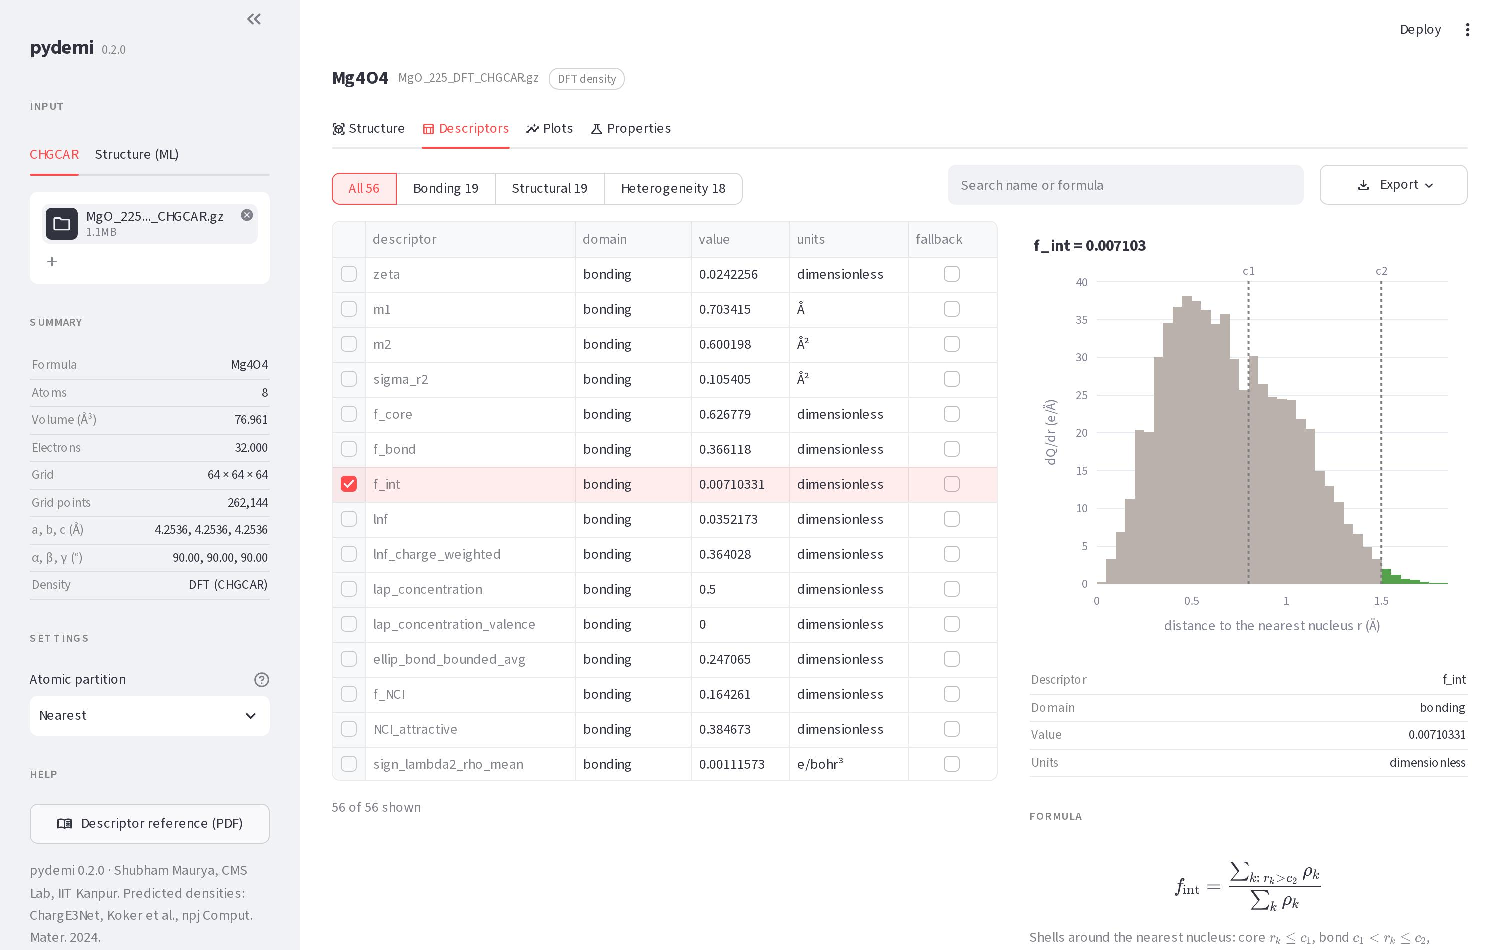
\includegraphics[width=\textwidth]{figures/fig_gui.pdf}
\caption{The graphical interface with the DFT \texttt{CHGCAR} of MgO (a
test-set structure), descriptor view: the 56 descriptors with the interstitial
charge fraction selected, its radial charge distribution with the shell
boundaries and its formula.}
\label{fig:gui}
\end{figure}

% ==========================================================================
\section{Conclusions}
\label{sec:conclusions}
pydemi reduces the one file every VASP calculation writes, the
\texttt{CHGCAR}, to 56 intensive and individually interpretable descriptors,
chosen so that each is defined on the PAW pseudo-density and converged on
typical grids: on a coarsened grid 46 of the 55 informative descriptors change
by at most 1\%. It featurized 6,059 VASP densities without a failure in
8.4 CPU hours and is verified by 352 tests. The included ChargE3Net model gives
the same descriptors from a crystal structure: 44 of the 55 keep a rank
correlation of at least 0.95 with their DFT values on 605 held-out structures,
and only the critical-point counts, quantities built on second derivatives in
low-density regions and descriptors with clustered values do not.

As the only inputs of gradient-boosted models, the descriptors predict 17
properties of the dataset, and for the elastic moduli they are on par with
graph neural networks trained on the same split and ahead of density-based
networks. The information is concentrated in a few simple, converged
descriptors, led by the interstitial density and the NCI volume:
ten descriptors per property retain 92--99\% of the test $R^2$ of all 55, and most of them transfer to ML-predicted densities. Because the property predictions from ML-predicted densities
are nearly as accurate as those from DFT densities, a structure suffices to
obtain both the descriptors and the properties, in seconds to minutes instead
of a DFT calculation. Models that predict the magnetization would extend this
path to magnetic descriptors.

\section*{Code and data availability}
The source code, the 352 tests, the descriptor reference and the scripts that
train the property models are available at
\url{https://github.com/CMSLabIITK/pydemi} under the MIT licence; the version described here, 0.2.1, is archived at
Zenodo~\cite{pydemi} (\doi{10.5281/zenodo.23736932}). The fine-tuned
ChargE3Net checkpoint and the property models are included in the package. The ChargE3Net code included in pydemi is
taken from \url{https://github.com/AIforGreatGood/charge3net} (MIT licence). The
DFT dataset of 6,059 charge densities was generated by members of the CMS Lab,
Department of Materials Science \& Engineering, IIT Kanpur, including the
authors, and was introduced in Ref.~\cite{kumar2026}; the data released with
that work are available at \url{https://github.com/CMSLabIITK/LatentMatFusion}.
The descriptors of all structures, the descriptors of the predicted test
densities, the property targets and the model results are included in the
repository. The DFT calculations themselves (about 180\,GB) are available from
the corresponding author upon reasonable request.

\section*{Acknowledgements}
We acknowledge the National Supercomputing Mission (NSM) for providing
computing resources of ``PARAM Sanganak'' at IIT Kanpur, which is implemented
by CDAC and supported by the Ministry of Electronics and Information Technology
(MeitY) and the Department of Science and Technology (DST), Government of
India. We also thank the ICME National Hub, IIT Kanpur, and CC, IIT Kanpur, for
providing an HPC facility.

\bibliographystyle{unsrt}
\bibliography{references}

\end{document}
